

\begin{table}[htbp]
\centering
\caption{Anti-Persona}
\label{tab:Table_persona4}
\small
\begin{tabular}{| m{0.2\textwidth} m{0.7\textwidth}|}
\hline \multicolumn{2}{|c|}{\textbf{Identidade}} \\ \hline
& \\

\begin{center} 
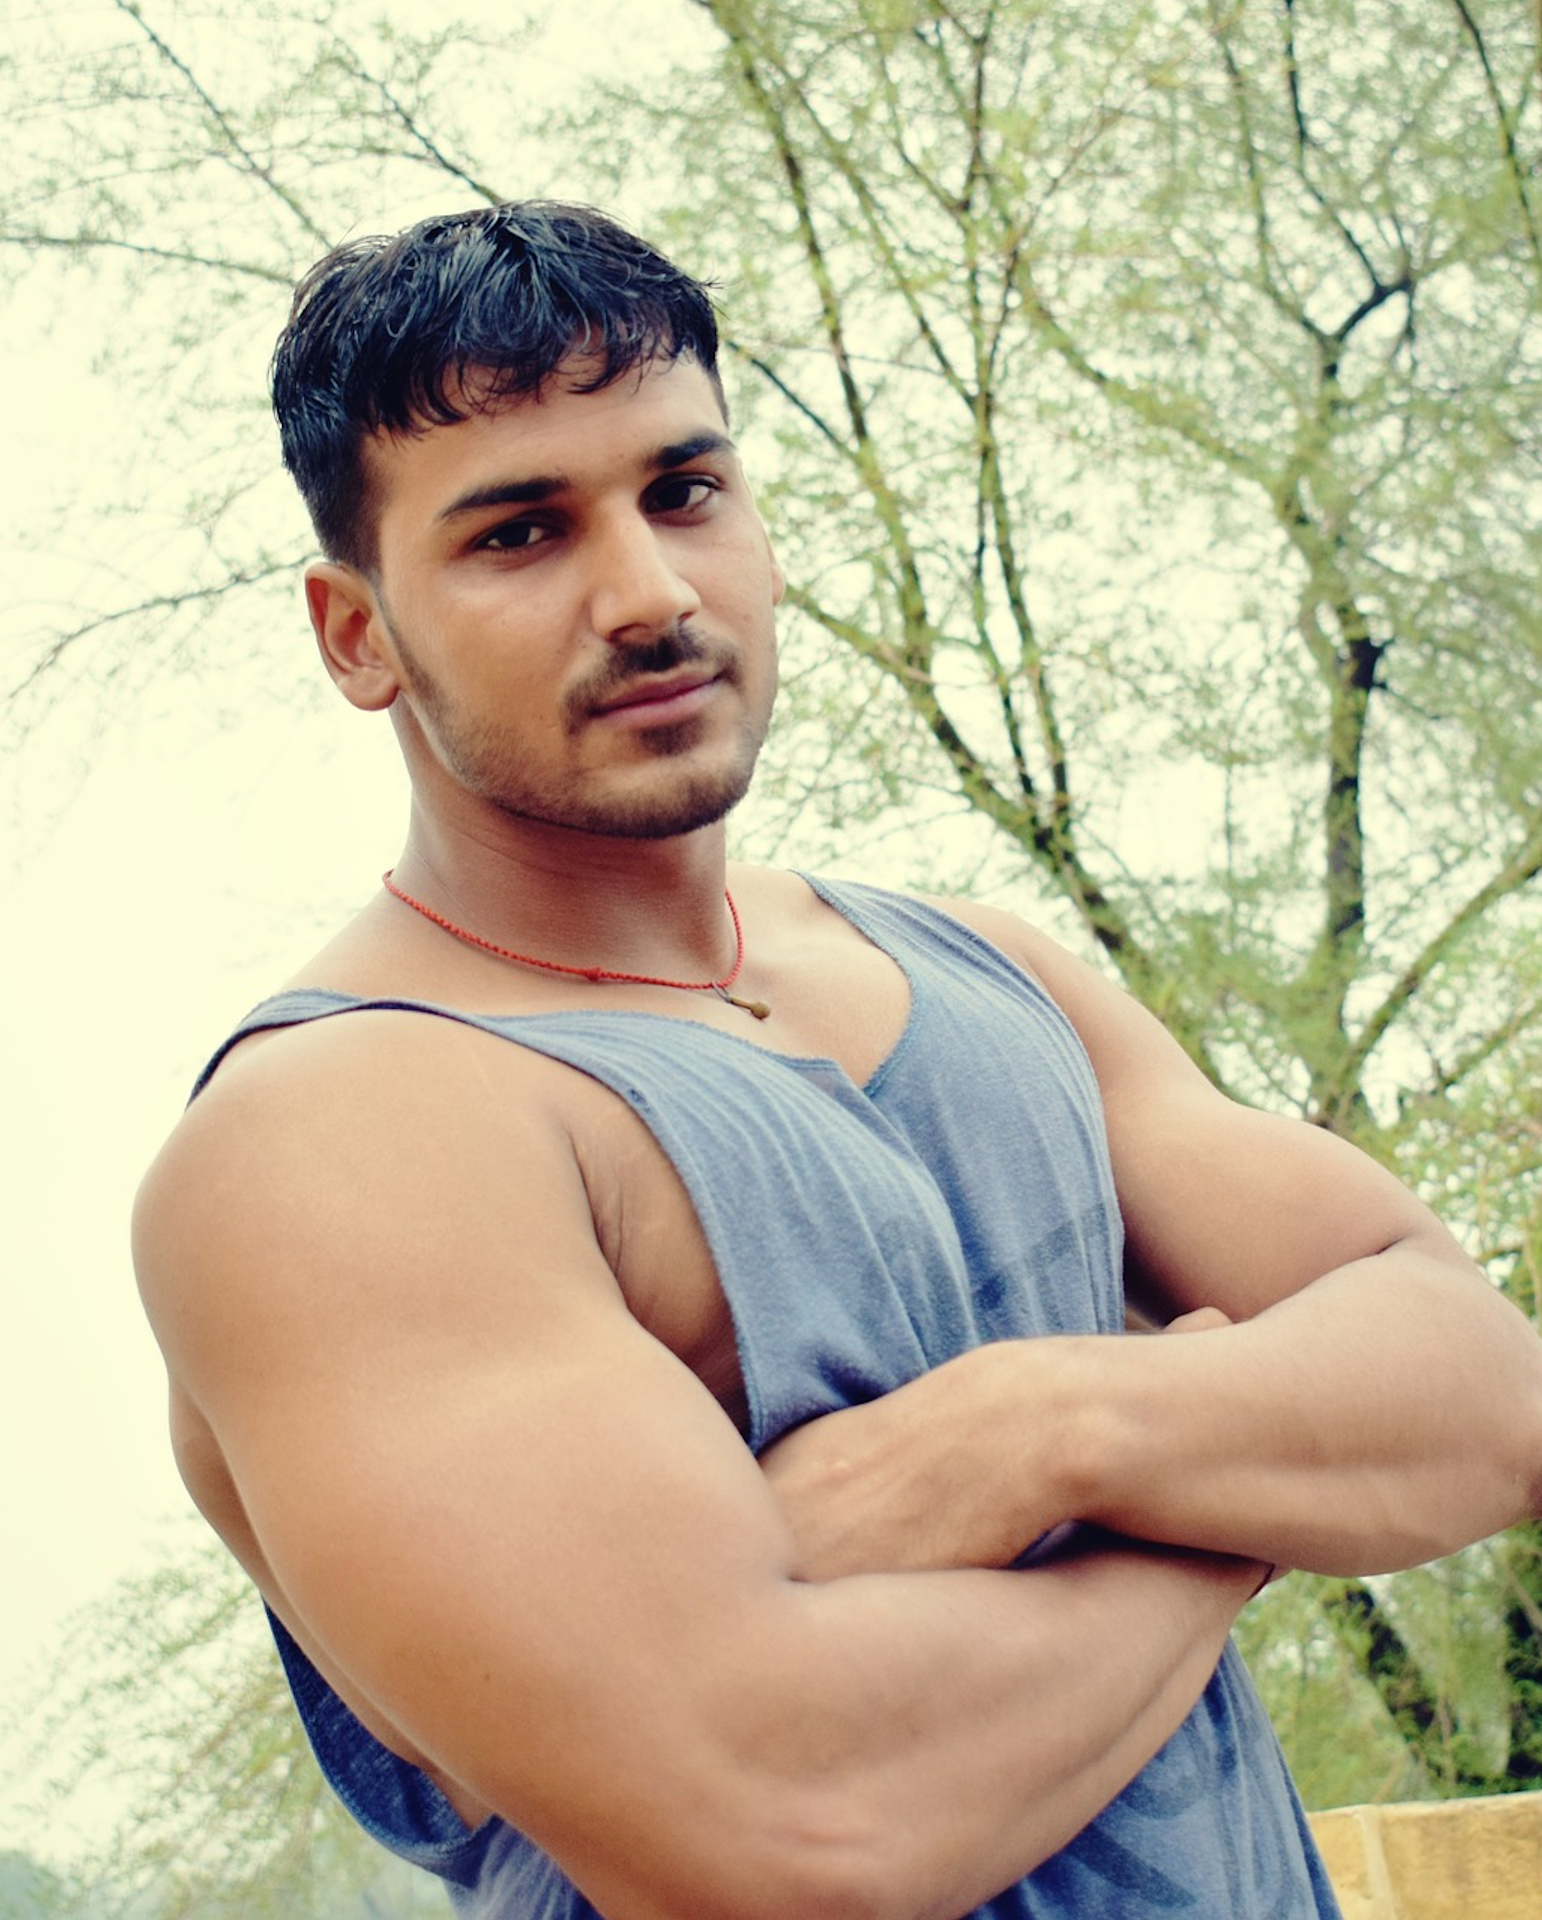
\includegraphics[scale=0.04]{figuras/personas/man-1209494_1920.jpg} 
Fonte: Pixabay\tablefootnote{https://pixabay.com/photos/biceps-aesthetics-body-fitness-2746490/}
\end{center} 

&

\textbf{Nome: }  Rafael Medeiros

\textbf{Idade:} 28 anos

\textbf{Ocupação:} Estudante de Educação Física na UnB - Darcy Ribeiro.

\\ \hline


\multicolumn{2}{|c|}{\textbf{Descrição Geral}} \\ \hline
\multicolumn{2}{|p{15cm}|}{
    \begin{tabular}[c]{@{}l@{}}\\
        Não tenho costume de usar jogos para aprendizagem, devo ter jogado uma vez ou outra,\\ mas\textbf{não me interessei muito} e rapidamente \textbf{o jogo se tornou monótono} pra mim e\\ isso me frustrou, pois não alcancei meu objetivo de estudo. Prefiro jogos esportivos como\\ futebol e basquete. Em relação ao conhecimento acadêmico, me concentro apenas nas\\ disciplinas do meu curso. \\
    \end{tabular}
}

\\ \hline
\multicolumn{2}{|c|}{\textbf{Aspectos de Qualidade}} \\ \hline

\multicolumn{2}{|p{15cm}|}{
    \begin{tabular}[c]{@{}l@{}}\\
        No geral, sou bem \textbf{competitivo}, ``dou o sangue'' para \textbf{conquistar} um gol e fazer um \\\textbf{ponto} em qualquer jogo. Em jogos digitais eu gosto de ser envolvido com uma \textbf{história} \\bacana e fico bastante empolgado com gráficos bem realistas e sofisticados. Sou mais fã \\de jogos com \textbf{trabalho em equipe} do que jogos individuais. Gosto tanto atividades \\ lúdicas que se desse pra aprender com elas, com certeza \textbf{trocaria qualquer livro} pra \\aprender me divertindo. \\
        \\
    \end{tabular}
} \\ \hline
\end{tabular}
\legend{Fonte: Autor}
\end{table}